\documentclass{article}
\usepackage{amsmath,amssymb,amsthm,kotex,mdframed,paralist}

\newcounter{num}
%\newcommand{\defi}[1]
%{\bigskip\noindent\refstepcounter{num}\textbf{정의 \arabic{num}) #1}\par}
%\newcommand{\theo}[1]
%{\bigskip\noindent\refstepcounter{num}\textbf{정리 \arabic{num}) #1}\par}
\newcommand{\exam}[1]
{\bigskip\noindent\refstepcounter{num}\textbf{예제 \arabic{num}) #1}\par}
\newcommand{\prob}[1]
{\bigskip\noindent\refstepcounter{num}\textbf{문제 \arabic{num}) #1}\par}
\newcommand{\summ}[1]
{\bigskip\noindent\refstepcounter{num}\textbf{요약 \arabic{num}) #1}\par}

\renewcommand{\figurename}{그림}
%\renewcommand{\proofname}{증명)}
\newcommand{\sol}{\par\bigskip\noindent{\bfseries풀이)}\par}
\newcommand{\ans}[1]{{\raggedleft\textbf{답 : }#1\par}}

%%%
\begin{document}

\title{혜령02 : 복습(2)}
\author{}
\date{\today}
\maketitle
\tableofcontents
\newpage

%%
\section{평행이동}
%
\exam{\(y\)축 방향의 평행이동}
직선 \(y=2x+1\)을 \(y\)축 방향으로 \(3\)만큼 평행이동해보자.
평행이동한 직선은 기울기는 \(2\)로 일정하지만 \(y\)절편이 \(1\)에서 \(3\)만큼 증가하여 \(4\)가 된다.
따라서 평행이동한 직선은 \(y=2x+4\)이 된다.

이처럼 단순히 \(y\)절편의 값에 \(3\)을 더해 \(y=2x+4\)를 얻었다고 볼 수도 있지만
\begin{align*}
y=2x+1\qquad
&\Longrightarrow\qquad y=(2x+1)+3\quad(\text{우변에 3을 더함.})\\
&\Longrightarrow\qquad y=2x+4
\end{align*}
\(y\) 대신 \(y-3\)을 대입해서 \(y=2x+4\)를 얻었다고 말해도 똑같은 설명이 된다는 점을 주목하자.
\begin{align*}
y=2x+1\qquad
&\Longrightarrow\qquad y-3=2x+1\quad(y\text{대신에 }y-3\text{를 대입.})\\
&\Longrightarrow\qquad y=2x+4
\end{align*}

%
\exam{\(x\)축 방향의 평행이동}
같은 직선을 \(x\)축 방향으로 \(2\)만큼 평행이동해보자.
평행이동한 직선의 기울기는 \(2\)로 일정하다.
\(y\)절편을 결정하기 위해서, \(y=2x+n\)라고 놓자.
원래 직선인 \(y=2x+1\)은 \((0,1)\)을 지나므로, 평행이동한 직선은 \((0,1)\)을 \(x\)축 방향으로 \(2\)만큼 평행이동한 \((2,1)\)을 지난다.
따라서 \(1=2\cdot2+n\)이고, \(n=-3\)이다.
따라서 평행이동한 직선은 \(y=2x-3\)이 된다.

위 방법은 분명히 사용 가능한 방법이지만, 약간 복잡하다.
아까 \(y\)축 방향으로 \(3\)만큼의 평행이동을 설명할 때에, \(y\) 대신 \(y-3\)을 대입하는 방법과 비슷한 방법을 적용해보면 어떨까?
\(x\)축 방향으로 \(2\)만큼의 평행이동이므로 \(x\)대신 \(x-3\)을 대입해보면
\begin{align*}
y=2x+1\qquad
&\Longrightarrow\qquad y=2(x-2)+1\quad(x\text{대신에 }x-2\text{를 대입.})\\
&\Longrightarrow\qquad y=2x-3
\end{align*}
이 되어 방금 전에 얻은 결과와 일치한다.
%이 결과들을 요약하면 다음과 같다.

%
\exam{\(x\)축, \(y\)축 방향의 평행이동}
이번에는 \(x\)축 방향으로의 평행이동과 \(y\)축 방향으로의 평행이동을 동시에 해보자.
\(y=2x+1\)을 \(x\)축 방향으로 \(2\)만큼, \(y\)축 방향으로 \(3\)만큼 평행이동하자.

먼저 \(x\)축 방향으로 \(2\)만큼 평행이동하면
\begin{align*}
y=2x+1\qquad
&\Longrightarrow\qquad y=2(x-2)+1\quad(x\text{대신에 }x-2\text{를 대입.})\\
&\Longrightarrow\qquad y=2x-3
\end{align*}
이고, 이것을 다시 \(y\)축 방향으로 \(3\)만큼 평행이동하면
\begin{align*}
y=2x-3\qquad
&\Longrightarrow\qquad y-3=2x-3\quad(y\text{대신에 }y-3\text{를 대입.})\\
&\Longrightarrow\qquad y=2x
\end{align*}
이다.

%한번에 설명할 수도 있다.
%\begin{align*}
%y=2x+1\qquad
%&\Longrightarrow\qquad y-3=2(x-2)+1\quad(x\text{대신에 }x-2\text{, }y\text{대신에 }y-3\text{대입.})\\
%&\Longrightarrow\qquad y=2x
%\end{align*}

%
\summ{평행이동}
\begin{enumerate}
\item
직선 \(y=ax+b\)를 \(x\)축 방향으로 \(m\)만큼, \(y\)축 방향으로 \(n\)만큼 평행이동한 직선의 식은 \(x\) 대신에 \(x-m\)를, \(y\) 대신에 \(y-n\)을 대입해 얻은 \(y-n=a(x-m)+b\)이다;
\begin{align*}
y=ax+b\qquad
&\Longrightarrow\qquad y=a(x-m)\quad(x\text{대신에 }x-m\text{을 대입.})\\
&\Longrightarrow\qquad y-n=a(x-m)\quad(y\text{대신에 }y-n\text{를 대입.})
\end{align*}
\item
일반적으로, 식 \(f(x,y)=0\)이 나타내는 도형을 \(x\)축 방향으로 \(m\)만큼, \(y\)축 방향으로 \(n\)만큼 평행이동한 도형이 나타내는 식은 \(x\) 대신에 \(x-m\)를, \(y\) 대신에 \(y-n\)을 대입해 얻은 \(f(x-m,y-n)=0\)이다;
\begin{align*}
f(x,y)=0\qquad
&\Longrightarrow\qquad f(x-m,y)=0\quad(x\text{대신에 }x-m\text{을 대입.})\\
&\Longrightarrow\qquad f(x-m,y-n)=0\quad(y\text{대신에 }y-n\text{를 대입.})
\end{align*}
\end{enumerate}

%
\prob{}
다음 식의 그래프를 평행이동한 그래프의 식을 구하고 모눈 위에 표시하여라.
\begin{enumerate}
\item
\(y=-2x+1\)를 \(x\)축 방향으로 \(4\)만큼 평행이동
\item
\(y=-2x+1\)를 \(y\)축 방향으로 \(-2\)만큼 평행이동
\item
\(y=-2x+1\)를 \(x\)축 방향으로 \(4\)만큼, \(y\)축 방향으로 \(-2\)만큼 평행이동
\end{enumerate}

%
\prob{}
다음 식의 그래프를 평행이동한 그래프의 식을 구하고 모눈 위에 표시하여라.
\begin{enumerate}
\item
\(y=\frac12x+1\)를 \(x\)축 방향으로 \(-2\)만큼 평행이동
\item
\(y=\frac12x+1\)를 \(y\)축 방향으로 \(3\)만큼 평행이동
\item
\(y=\frac12x+1\)를 \(x\)축 방향으로 \(-2\)만큼, \(y\)축 방향으로 \(3\)만큼 평행이동
\end{enumerate}

%
\prob{}
다음 식의 그래프를 평행이동한 그래프의 식을 구하고 모눈 위에 표시하여라.
\begin{enumerate}
\item
\(y=3x+1\)를 \(x\)축 방향으로 \(1\)만큼 평행이동
\item
\(y=3x+1\)를 \(y\)축 방향으로 \(3\)만큼 평행이동
\item
\(y=3x+1\)를 \(x\)축 방향으로 \(1\)만큼, \(y\)축 방향으로 \(3\)만큼 평행이동
\end{enumerate}

%
\prob{}
다음 식의 그래프를 평행이동한 그래프의 식을 구하고 모눈 위에 표시하여라.
\begin{enumerate}
\item
\(xy=1\)을 \(x\)축 방향으로 \(1\)만큼, \(y\)축 방향으로 \(2\)만큼 평행이동
\item
\(y=2^x\)을 \(x\)축 방향으로 \(-2\)만큼, \(y\)축 방향으로 \(3\)만큼 평행이동
\end{enumerate}

%%
\section{이차함수}

%
\summ{이차함수의 기본형}
\(y=ax^2\)의 그래프는 \(y=ax^2\)을 만족하는 모든 점들 \((x,y)\)의 집합으로 꼭지점이 \((0,0)\)인 포물선이다.
\(a>0\)이면 아래로 볼록한 포물선이고, \(a<0\)이면 위로 볼록한 포물선이다.

\begin{figure}[h!]
\centering
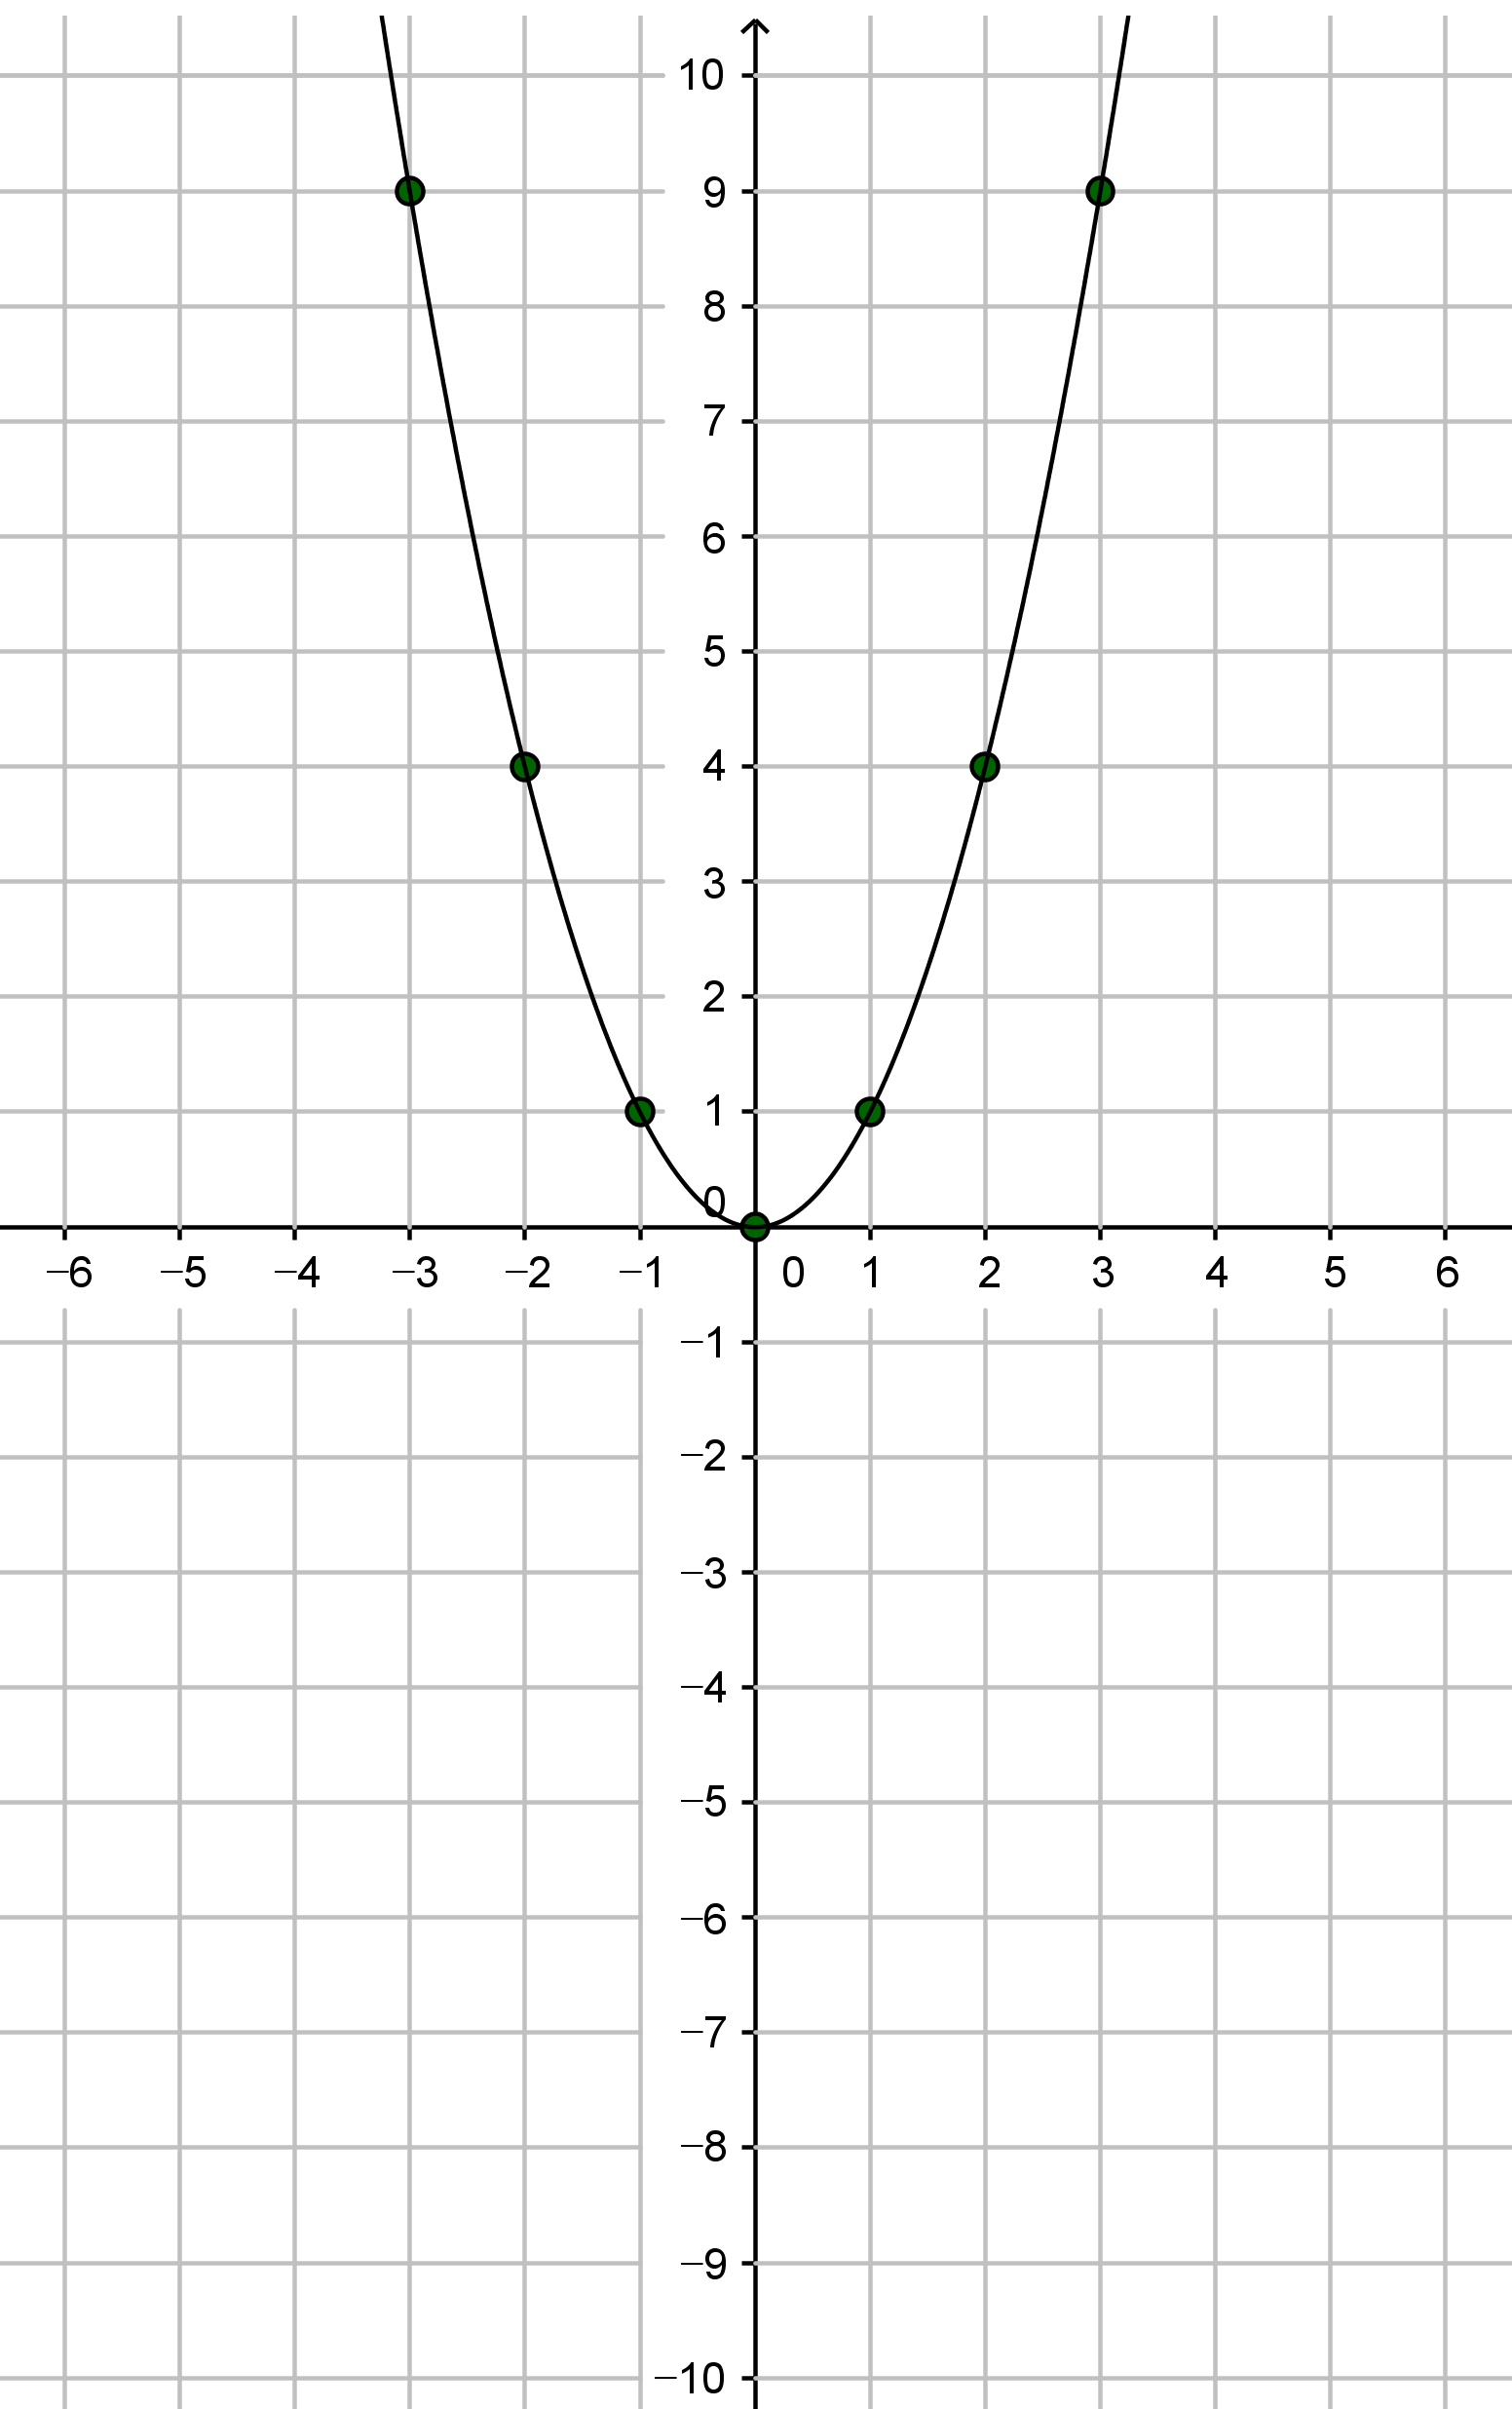
\includegraphics[width=0.3\textwidth]{y=x^2}
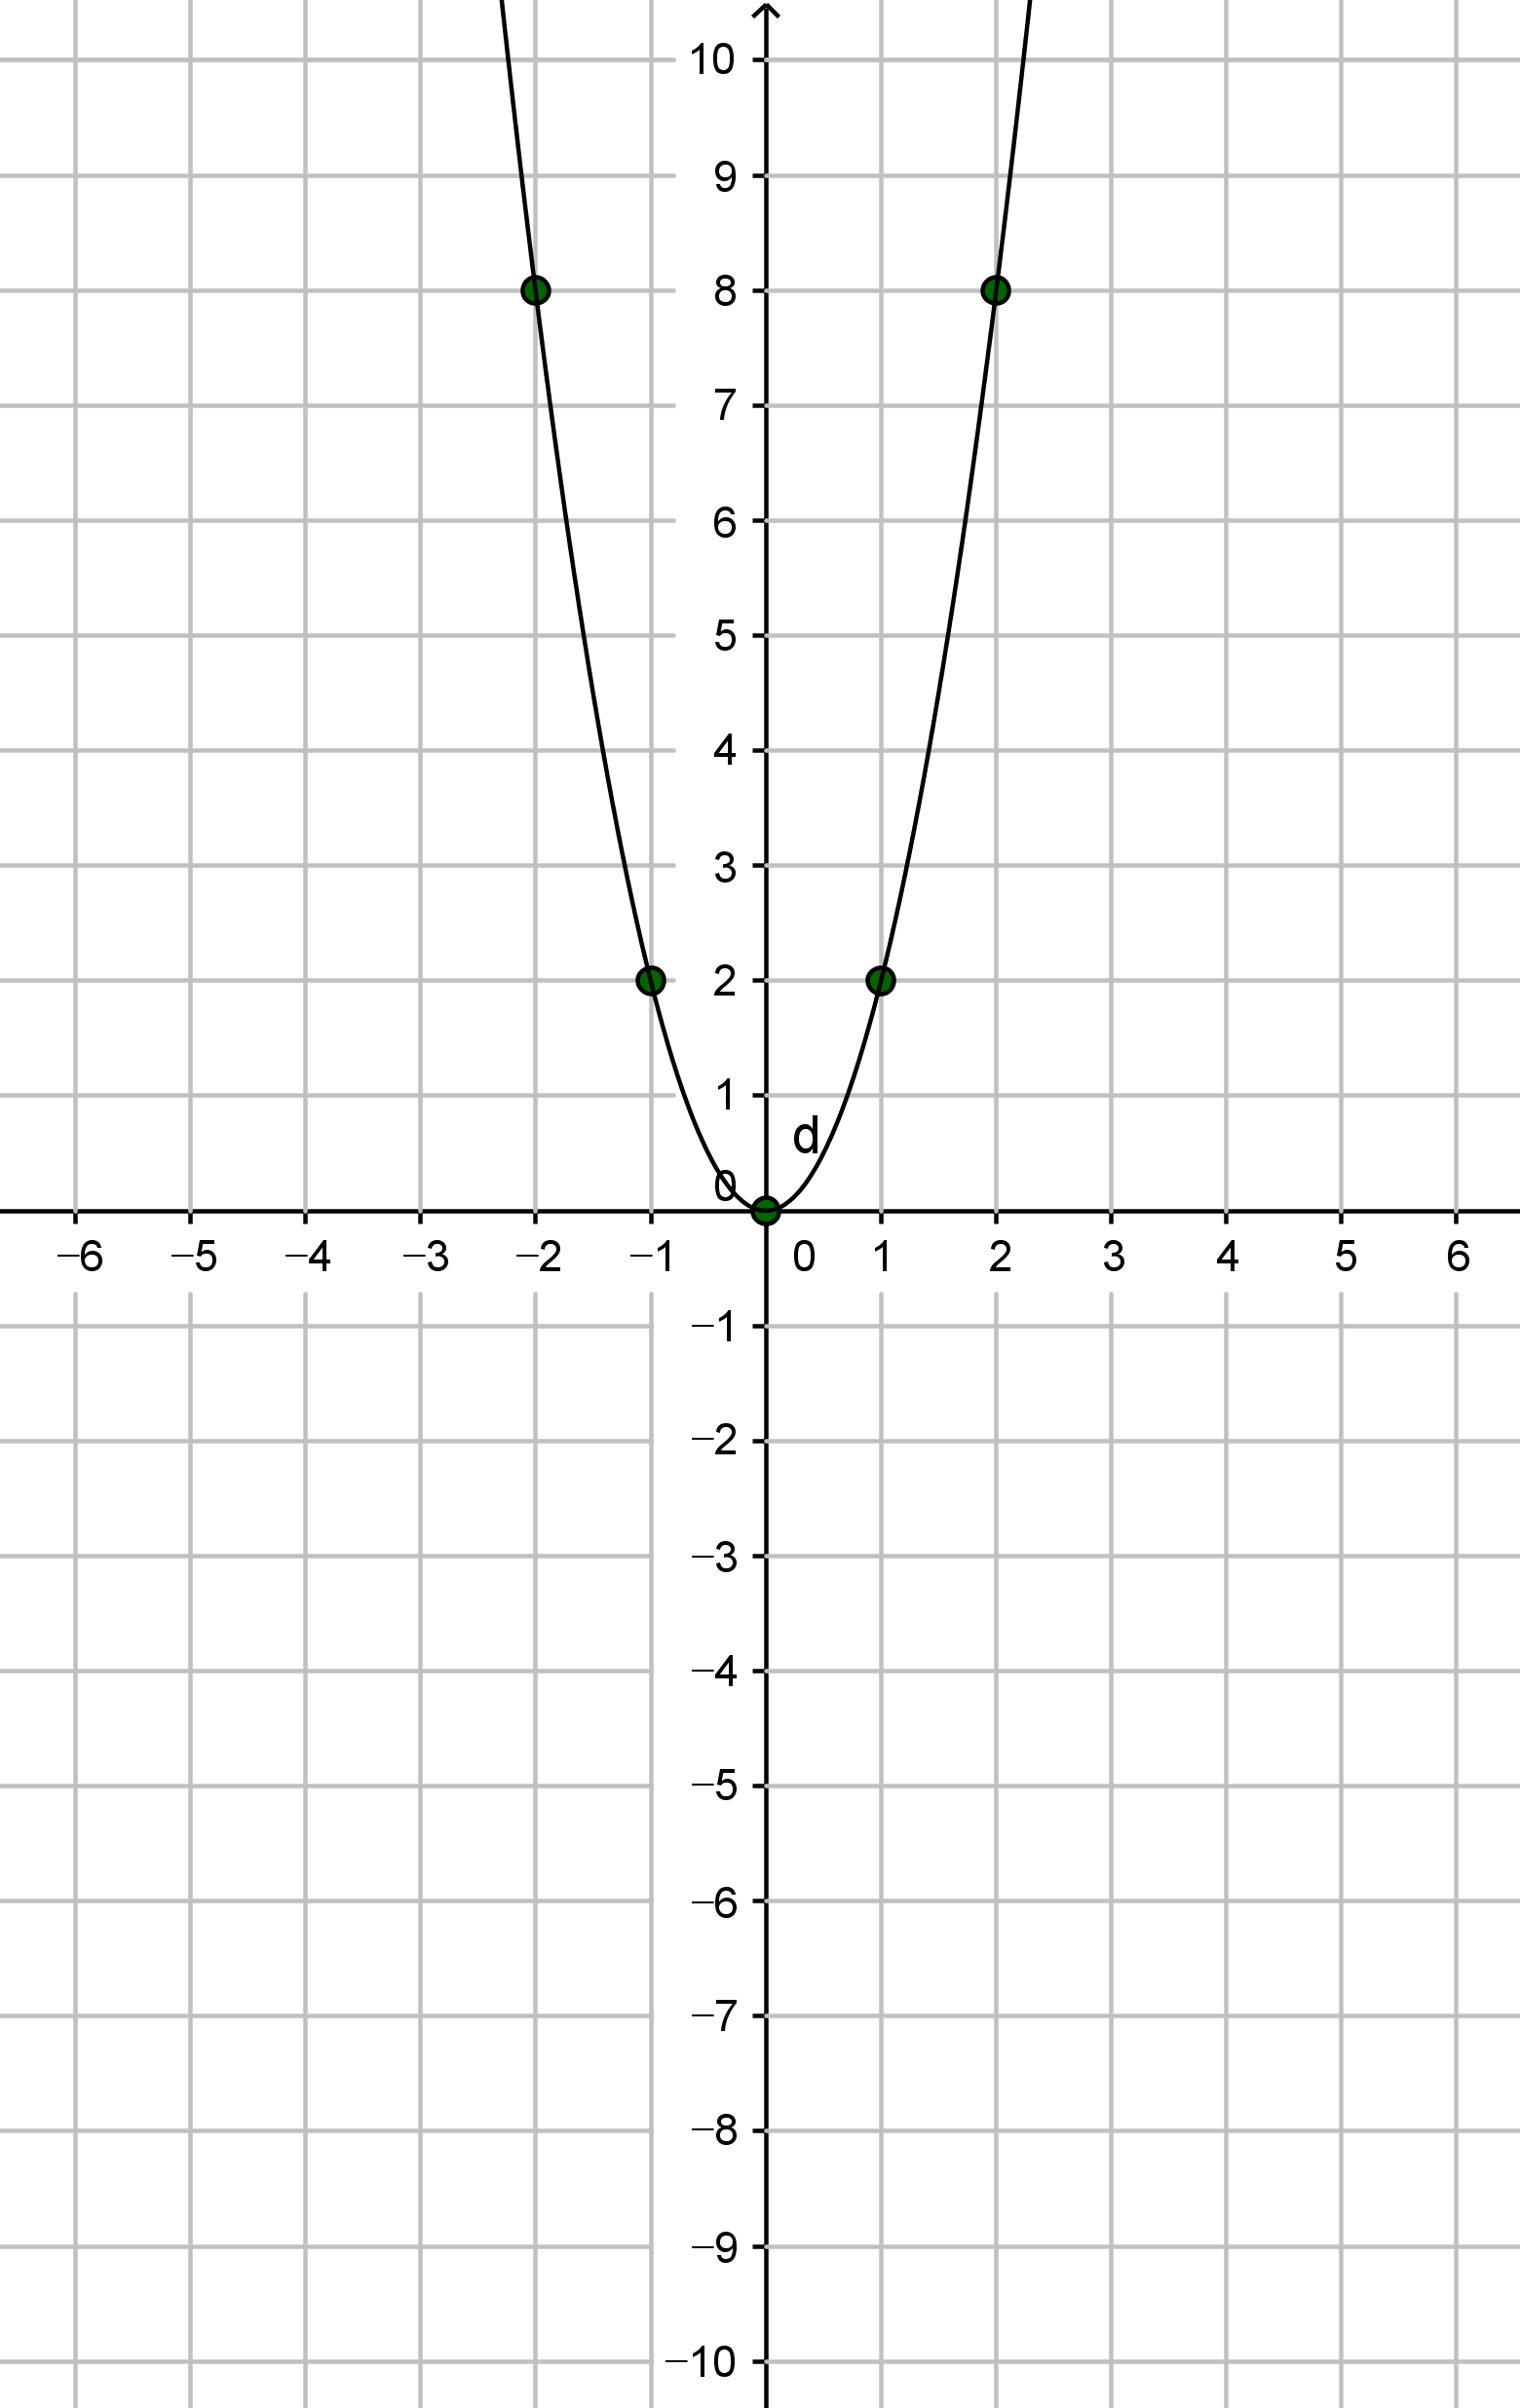
\includegraphics[width=0.3\textwidth]{y=2x^2}
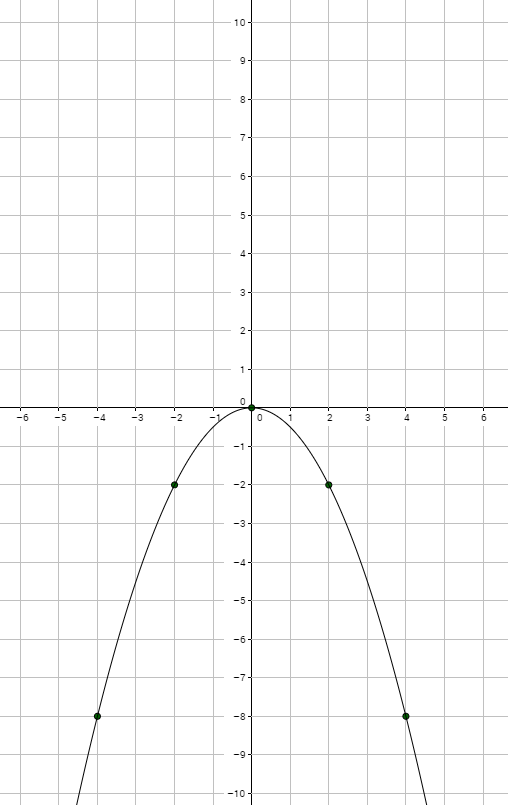
\includegraphics[width=0.3\textwidth]{y=-onehalfx^2}\\
\(y=x^2\)
\qquad\qquad\qquad\quad
\(y=2x^2\)
\qquad\qquad\qquad\quad
\(y=-\frac12x^2\)
\end{figure}

%
\summ{이차함수의 일반형}
이차함수
\[y=ax^2+bx+c,\quad(a\neq0)\]
는 적절한 계산을 통해
\[y=a(x-m)^2+n\]
꼴로 바꿀 수 있다.
이 함수의 그래프는 \(y=ax^2\)의 그래프를 \(x\)축 방향으로 \(m\)만큼, \(y\)축 방향으로 \(n\)만큼 평행이동하여 얻을 수 있다.

\exam{}
예를 들어 이차함수
\[y=2x^2+4x+3\]
의 그래프를 그리기 위해서는
\begin{align*}
y
&=2x^2+4x+3\\
&=2(x^2+2x)+3\\
&=2(x^2+2x+1-1)+3\\
&=2(x+1)^2+1
\end{align*}
와 같이 식을 변환하여
\[y=2(x+1)^2+1\]
를 얻고, \(y=2x^2\)의 그래프 그려, 이것을 \(x\)축 방향으로 \(-1\)만큼, \(y\)축 방향으로 \(1\)만큼 평행이동하면 된다.
\begin{figure}[h!]
\centering
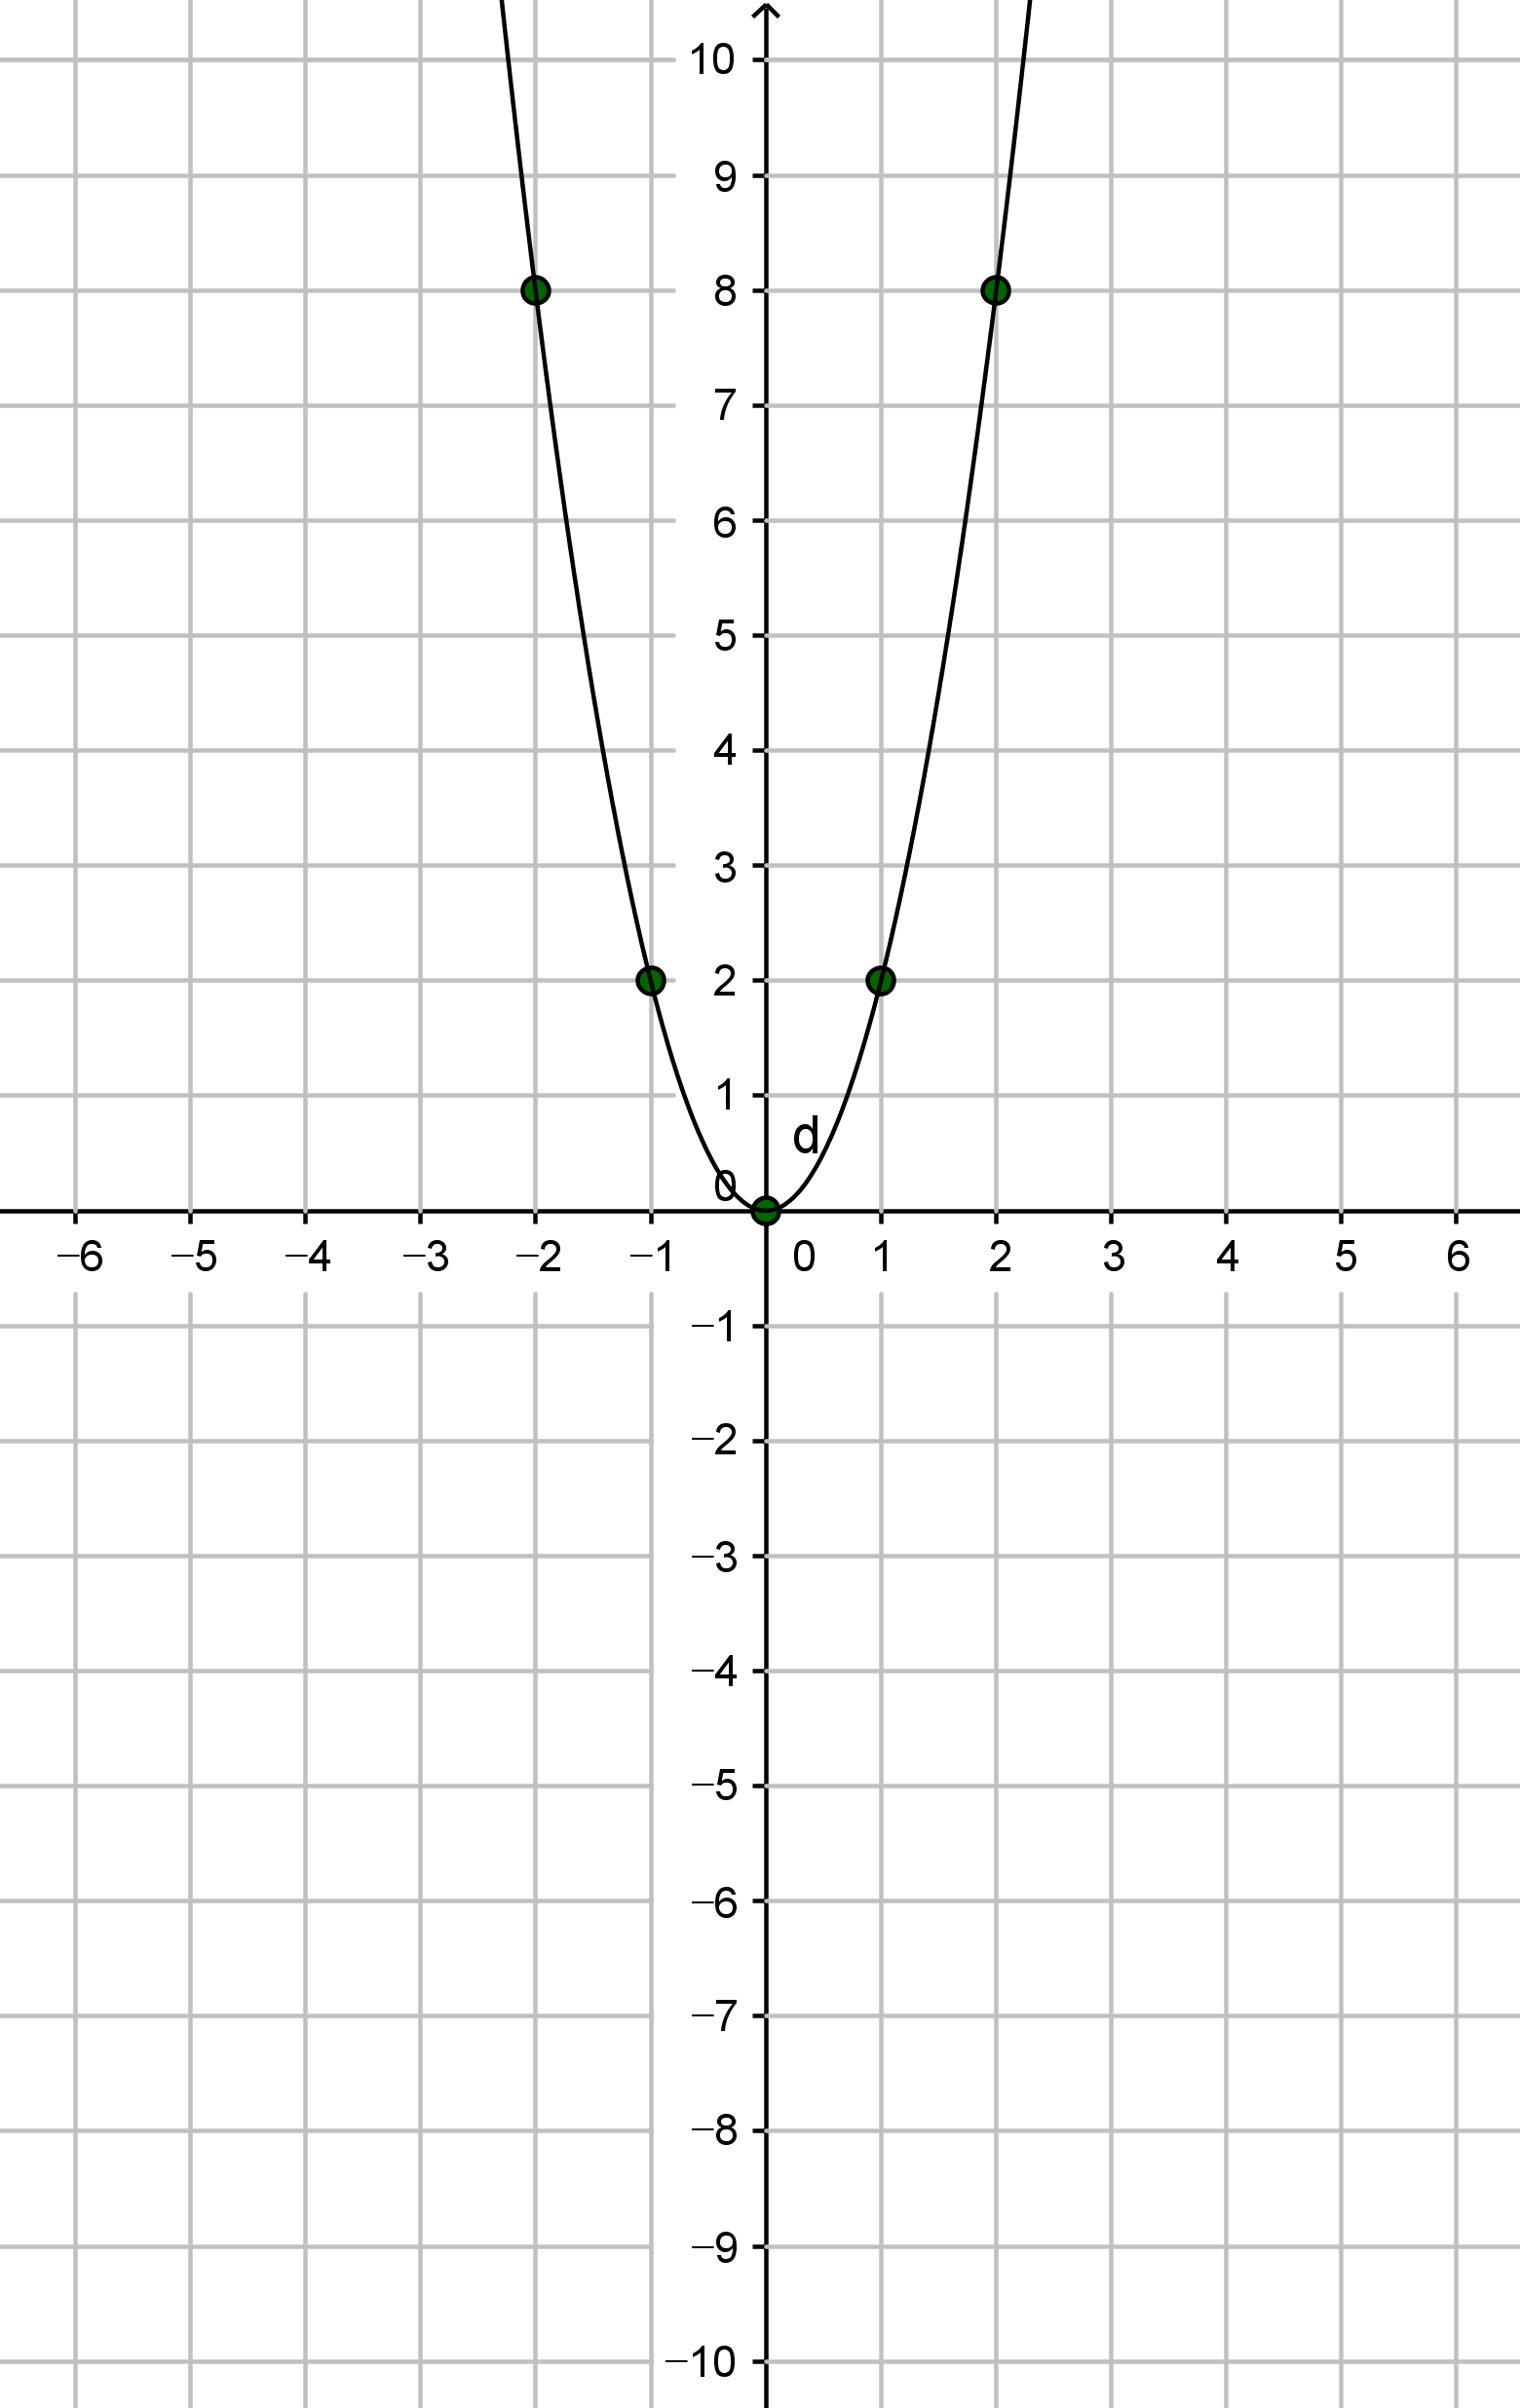
\includegraphics[width=0.3\textwidth]{y=2x^2}
\qquad\qquad
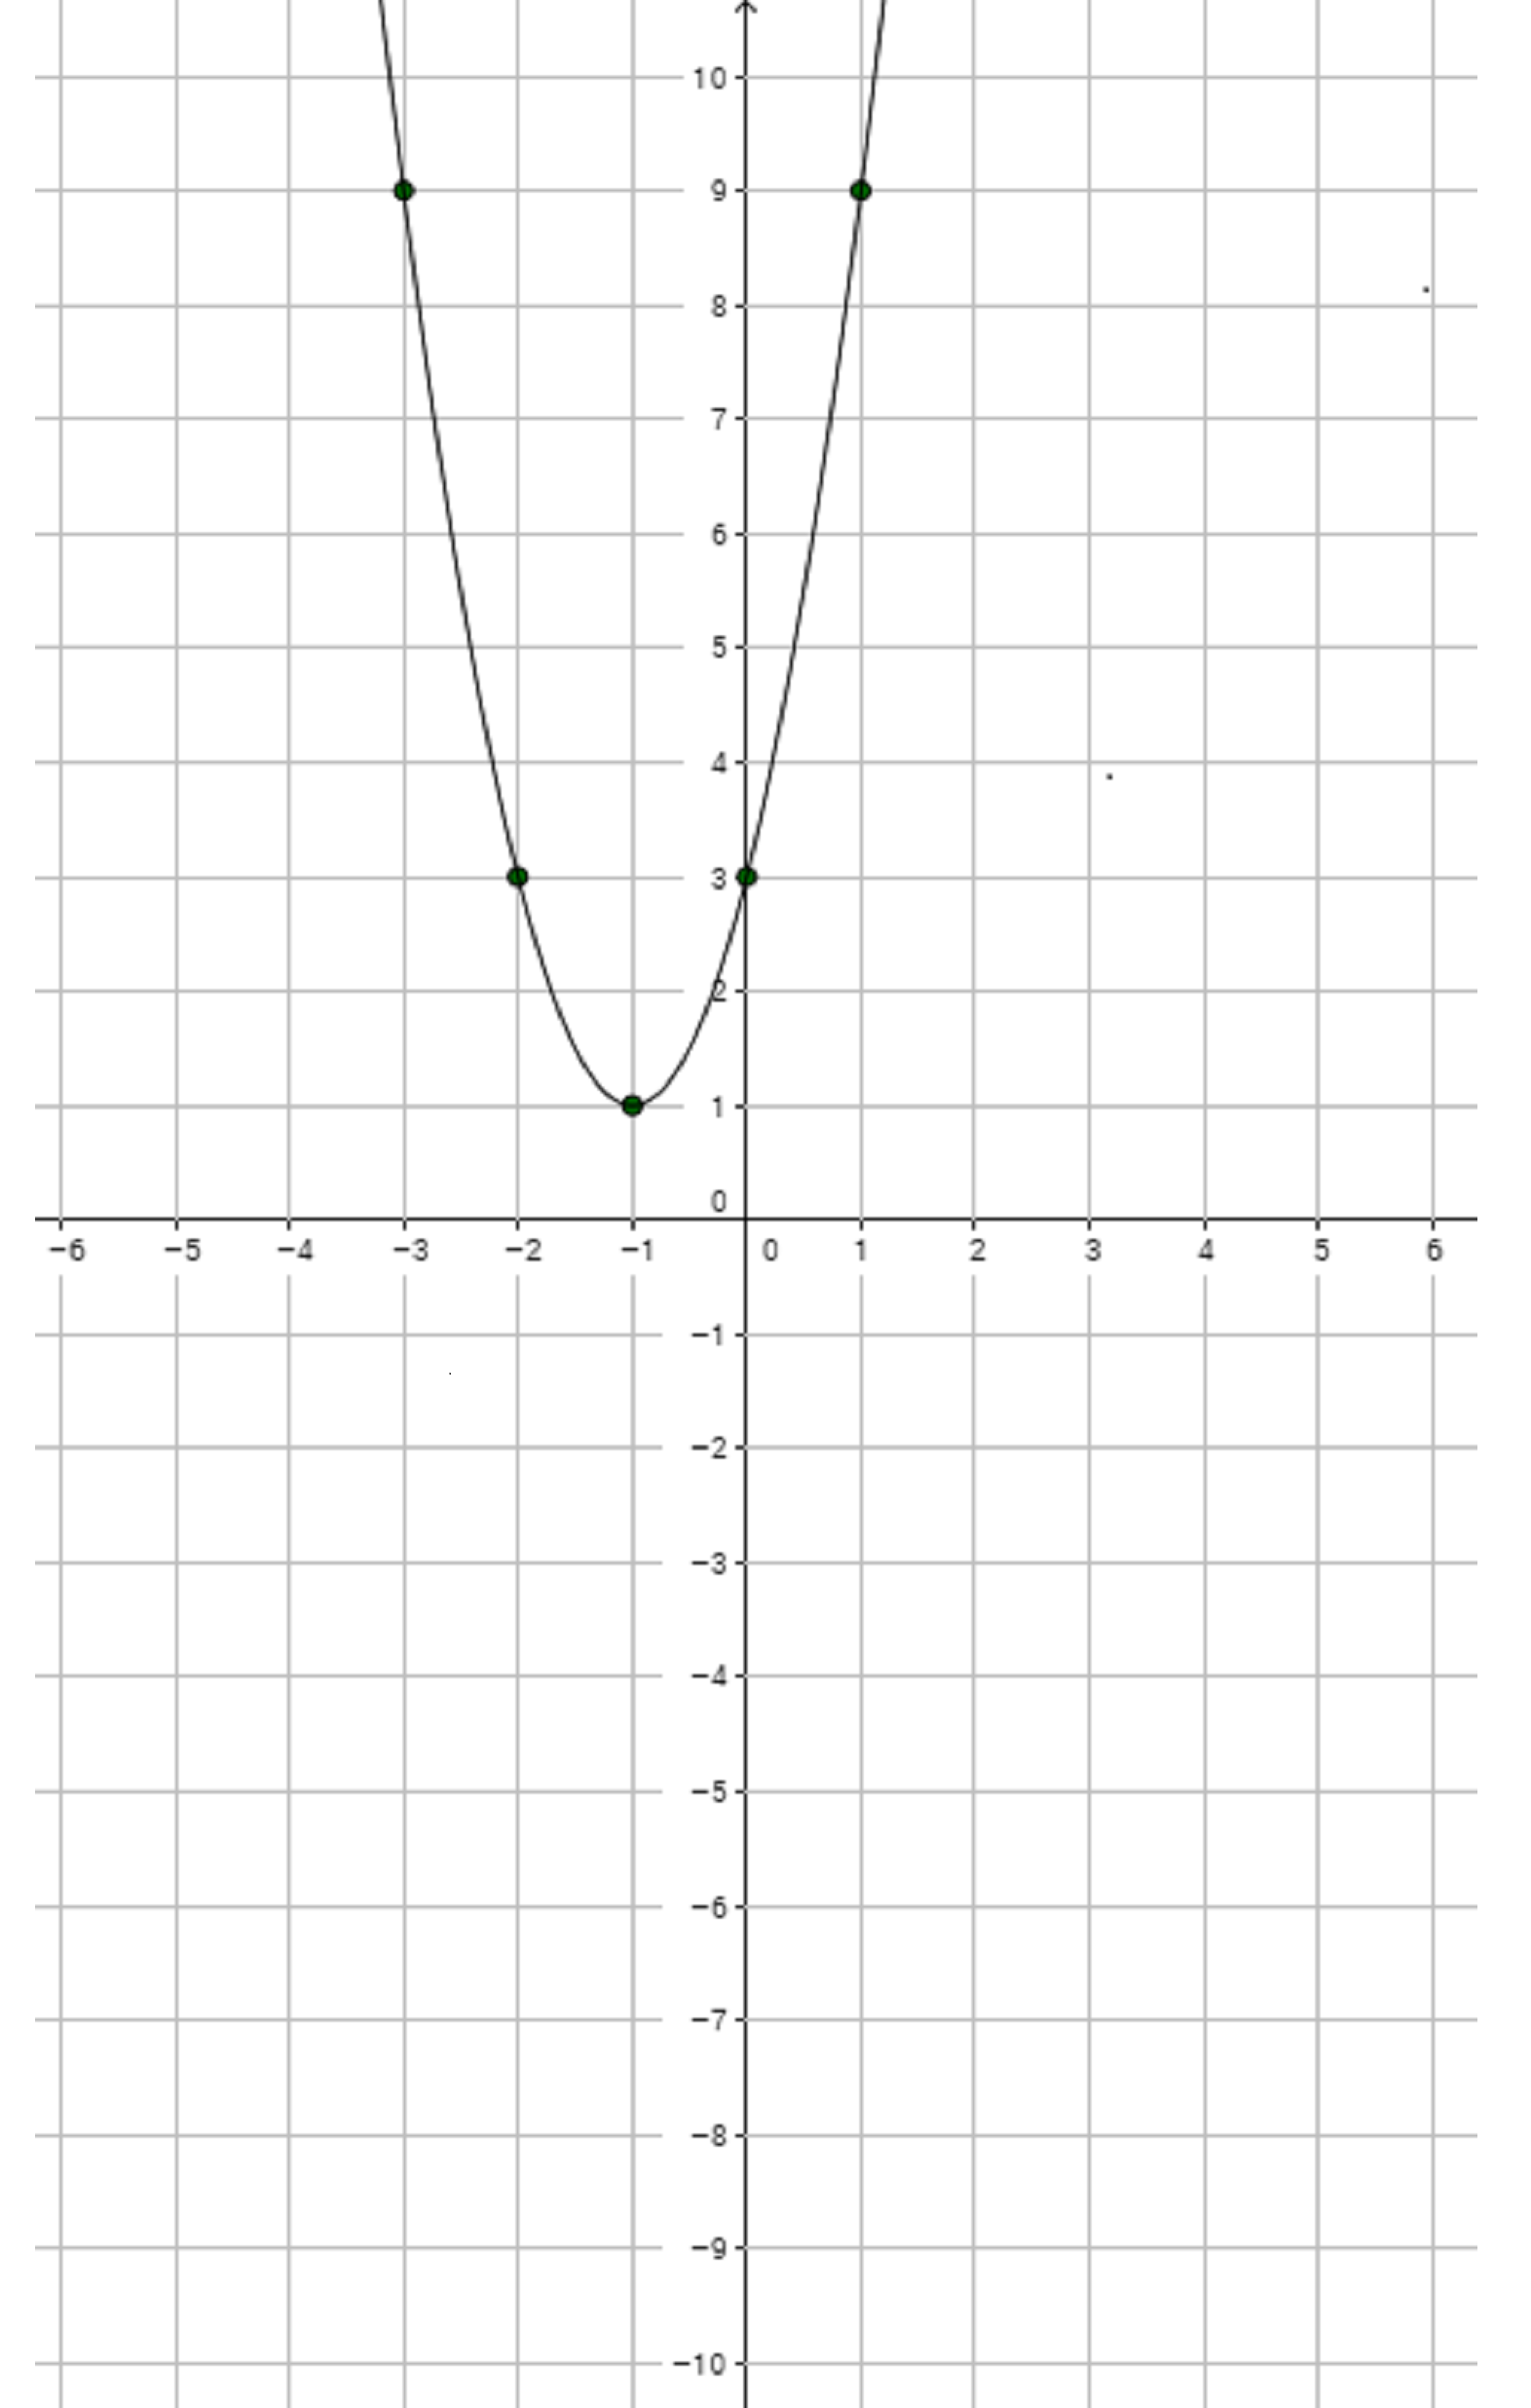
\includegraphics[width=0.3\textwidth]{y=2x^2+4x+3}\\
\qquad\(y=2x^2\)\qquad\qquad\qquad\qquad\(y=2x^2+4x+3\)
\end{figure}

%
\prob{}
다음 식의 그래프를 그리고, 그래프 위의 다섯 개 점(정수,정수)을 표시하시오.
\begin{enumerate}
\item
\(y=-x^2\)
\item
\(y=x^2-4x+3\)
\item
\(y=-2x^2+8x-5\)
\item
\(y=\frac12x^2+x+\frac32\)
\item
\(y=x^2+x+1\)
\end{enumerate}

\newpage
%%
\section{원}

%
\summ{원의 방정식의 기본형}
\(x^2+y^2=r^2\)의 그래프는 \(x^2+y^2=r^2\)을 만족하는 모든 점들 \((x,y)\)의 집합이다.
\(P=(x,y)\)라고 가정할 때 이 식은 정확히
\[\overline{PO}=r\]
이므로 이 식의 그래프는 중심이 원점이고 반지름이 \(r\)인 원이다.

\begin{figure}[h!]
\centering
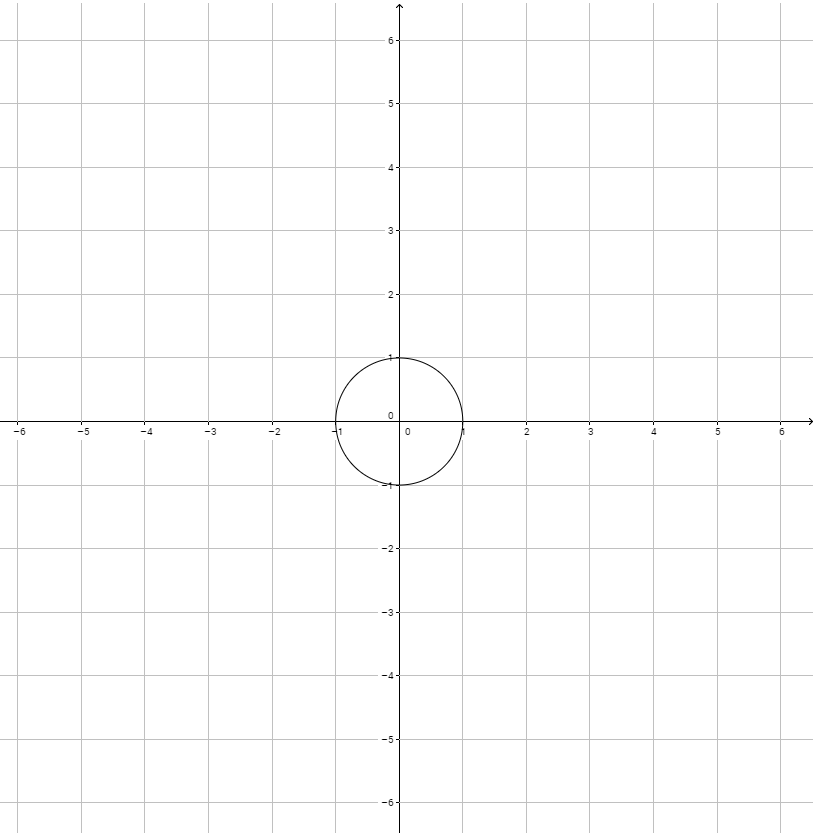
\includegraphics[width=0.4\textwidth]{x^2+y^2=1}
\qquad\quad
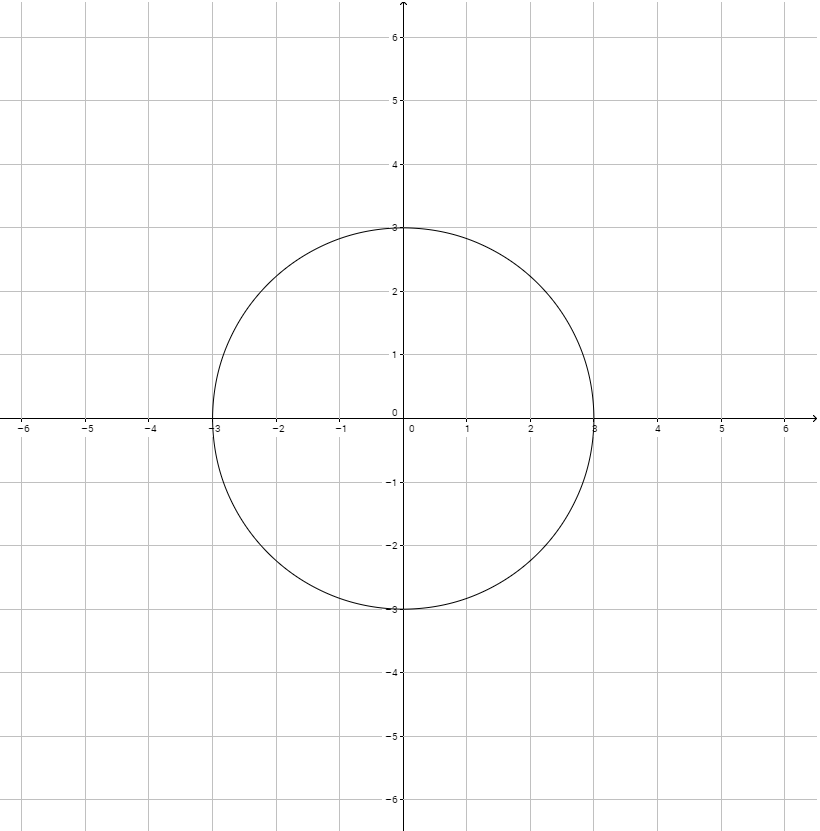
\includegraphics[width=0.4\textwidth]{x^2+y^2=9}\\
\(x^2+y^2=1\)
\qquad\qquad\qquad\quad\qquad\qquad
\(x^2+y^2=9\)
\end{figure}

%
\summ{원의 방정식의 일반형}
방정식
\[x^2+y^2+Ax+By+C\]
는 적절한 계산을 통해
\[(x-m)^2+(y-n)^2=r^2\]
꼴로 바꿀 수 있다.
이 함수의 그래프는 \(x^2+y^2=r^2\)의 그래프를 \(x\)축 방향으로 \(m\)만큼, \(y\)축 방향으로 \(n\)만큼 평행이동하여 얻을 수 있다.

\exam{}
예를 들어 방정식
\[x^2+2x+y^2-4y-4=0\]
의 그래프를 그리기 위해서는
\begin{align*}
&x^2+2x+y^2-4y-4=0\\
&(x^2+2x+1)-1+(y^2-4y+4)-4-4=0\\
&(x+1)^2+(y-2)^2=9
\end{align*}
와 같이 식을 변환하고, \(x^2+y^2=9\)의 그래프 그려, 이것을 \(x\)축 방향으로 \(-1\)만큼, \(y\)축 방향으로 \(2\)만큼 평행이동하면 된다.
\begin{figure}[h!]
\centering
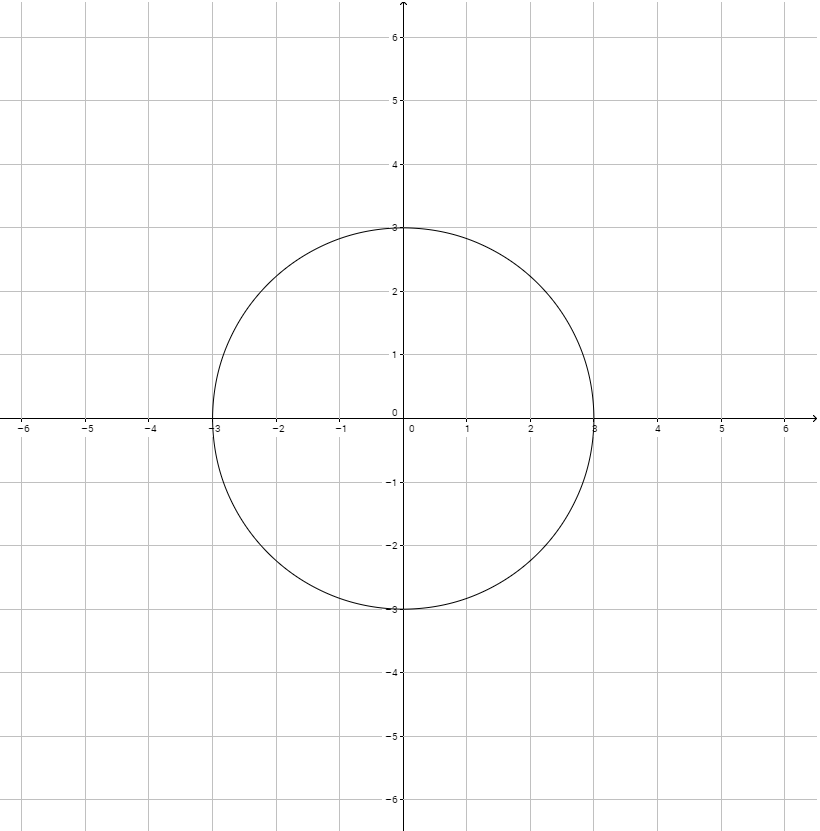
\includegraphics[width=0.4\textwidth]{x^2+y^2=9}
\qquad\qquad
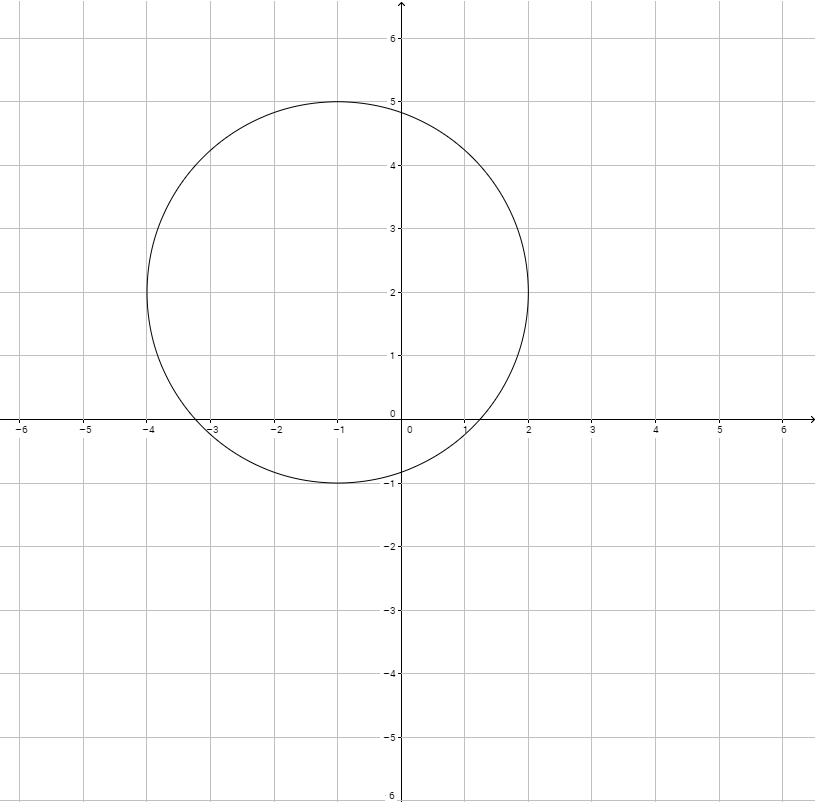
\includegraphics[width=0.4\textwidth]{x^2+2x+y^2-4y-4=0}\\
\qquad\(y=2x^2\)\qquad\qquad\qquad\qquad\qquad\(x^2+2x+y^2-4y-4=0\)
\end{figure}

%
\prob{}
다음 식의 그래프를 그리고, (정수,정수)점을 모두 표시하시오.
\begin{enumerate}
\item
\(x^2+y^2-6x+2y+5=0\)
\item
\(x^2+y^2-4x=0\)
\end{enumerate}

\newpage
%%
\section{두 도형 사이의 교점}
%
\exam{}
두 도형이 서로 만나는 점은 두 도형이 나타내는 식을 서로 연립하여 구한다.
예를 들어 포물선 \(y=x^2\)과 원 \(x^2+y^2+6x-8y=0\) 사이의 교점을 구해보자.
이것은 연립방정식
\[\begin{cases}
y=x^2\\
x^2+y^2+6x-8y=0
\end{cases}\]
을 풀어서 해결할 수 있다.

첫 번째 식을 두 번째 식에 대입해 정리하면
\begin{align*}
&x^4+(x^2)^2+6x-8x^2=0\\
&x^4-7x^2+6x=0\\
&x(x^3-7x+6)=0\\
&x(x-1)(x^2+x-6)=0\\
&x(x-1)(x-2)(x+3)=0\\
&x=-3,0,1,2
\end{align*}
이다.
따라서 가능한 \((x,y)\)는 \((x,y)=(-3,9),(0,0),(1,1),(2,4)\)이다.
\begin{figure}[h!]
\centering
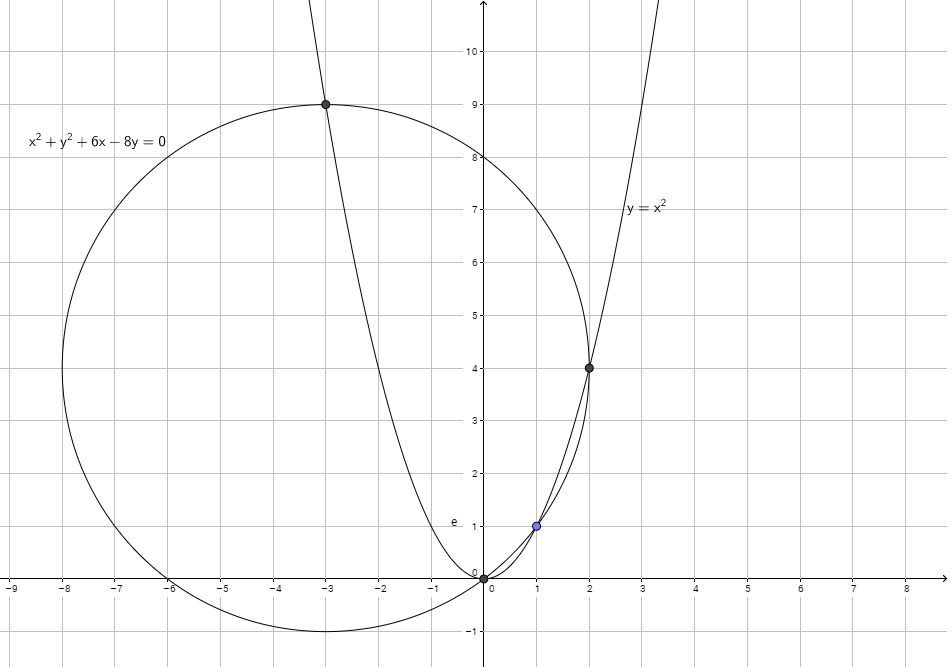
\includegraphics[width=0.9\textwidth]{intersects}
\end{figure}

%
\prob{}
다음 식이 나타내는 도형들의 교점의 좌표를 모두 구하시오.
\begin{enumerate}
\item
\(y=x^2\), \(x+y=2\)
\item
\(y=x^2+1\), \(x+2y=4\)
\item
\(x^2+y^2=25\), \(y=x+1\)
\item
\(x^2+y^2+4x-2y-12=0\), \(y=x^2-4\)
\end{enumerate}

%
\prob{}
이차함수 \(2x^2-3x+1\)의 그래프와 직선 \(y=x+k\)가 서로 접하기 위한 \(k\)의 값을 구하시오.
\end{document}